\label{sec:RESULTS}
In section \ref{sec:INTRO}, we discussed the principal fields that can benefit from optical metrology. In order to encompass the majority of the fields in the experimental section, the team decided to reconstruct a polystyrene bust as shown in figure \ref{fig:Bust}.
\begin{figure}[H]
    \centering
    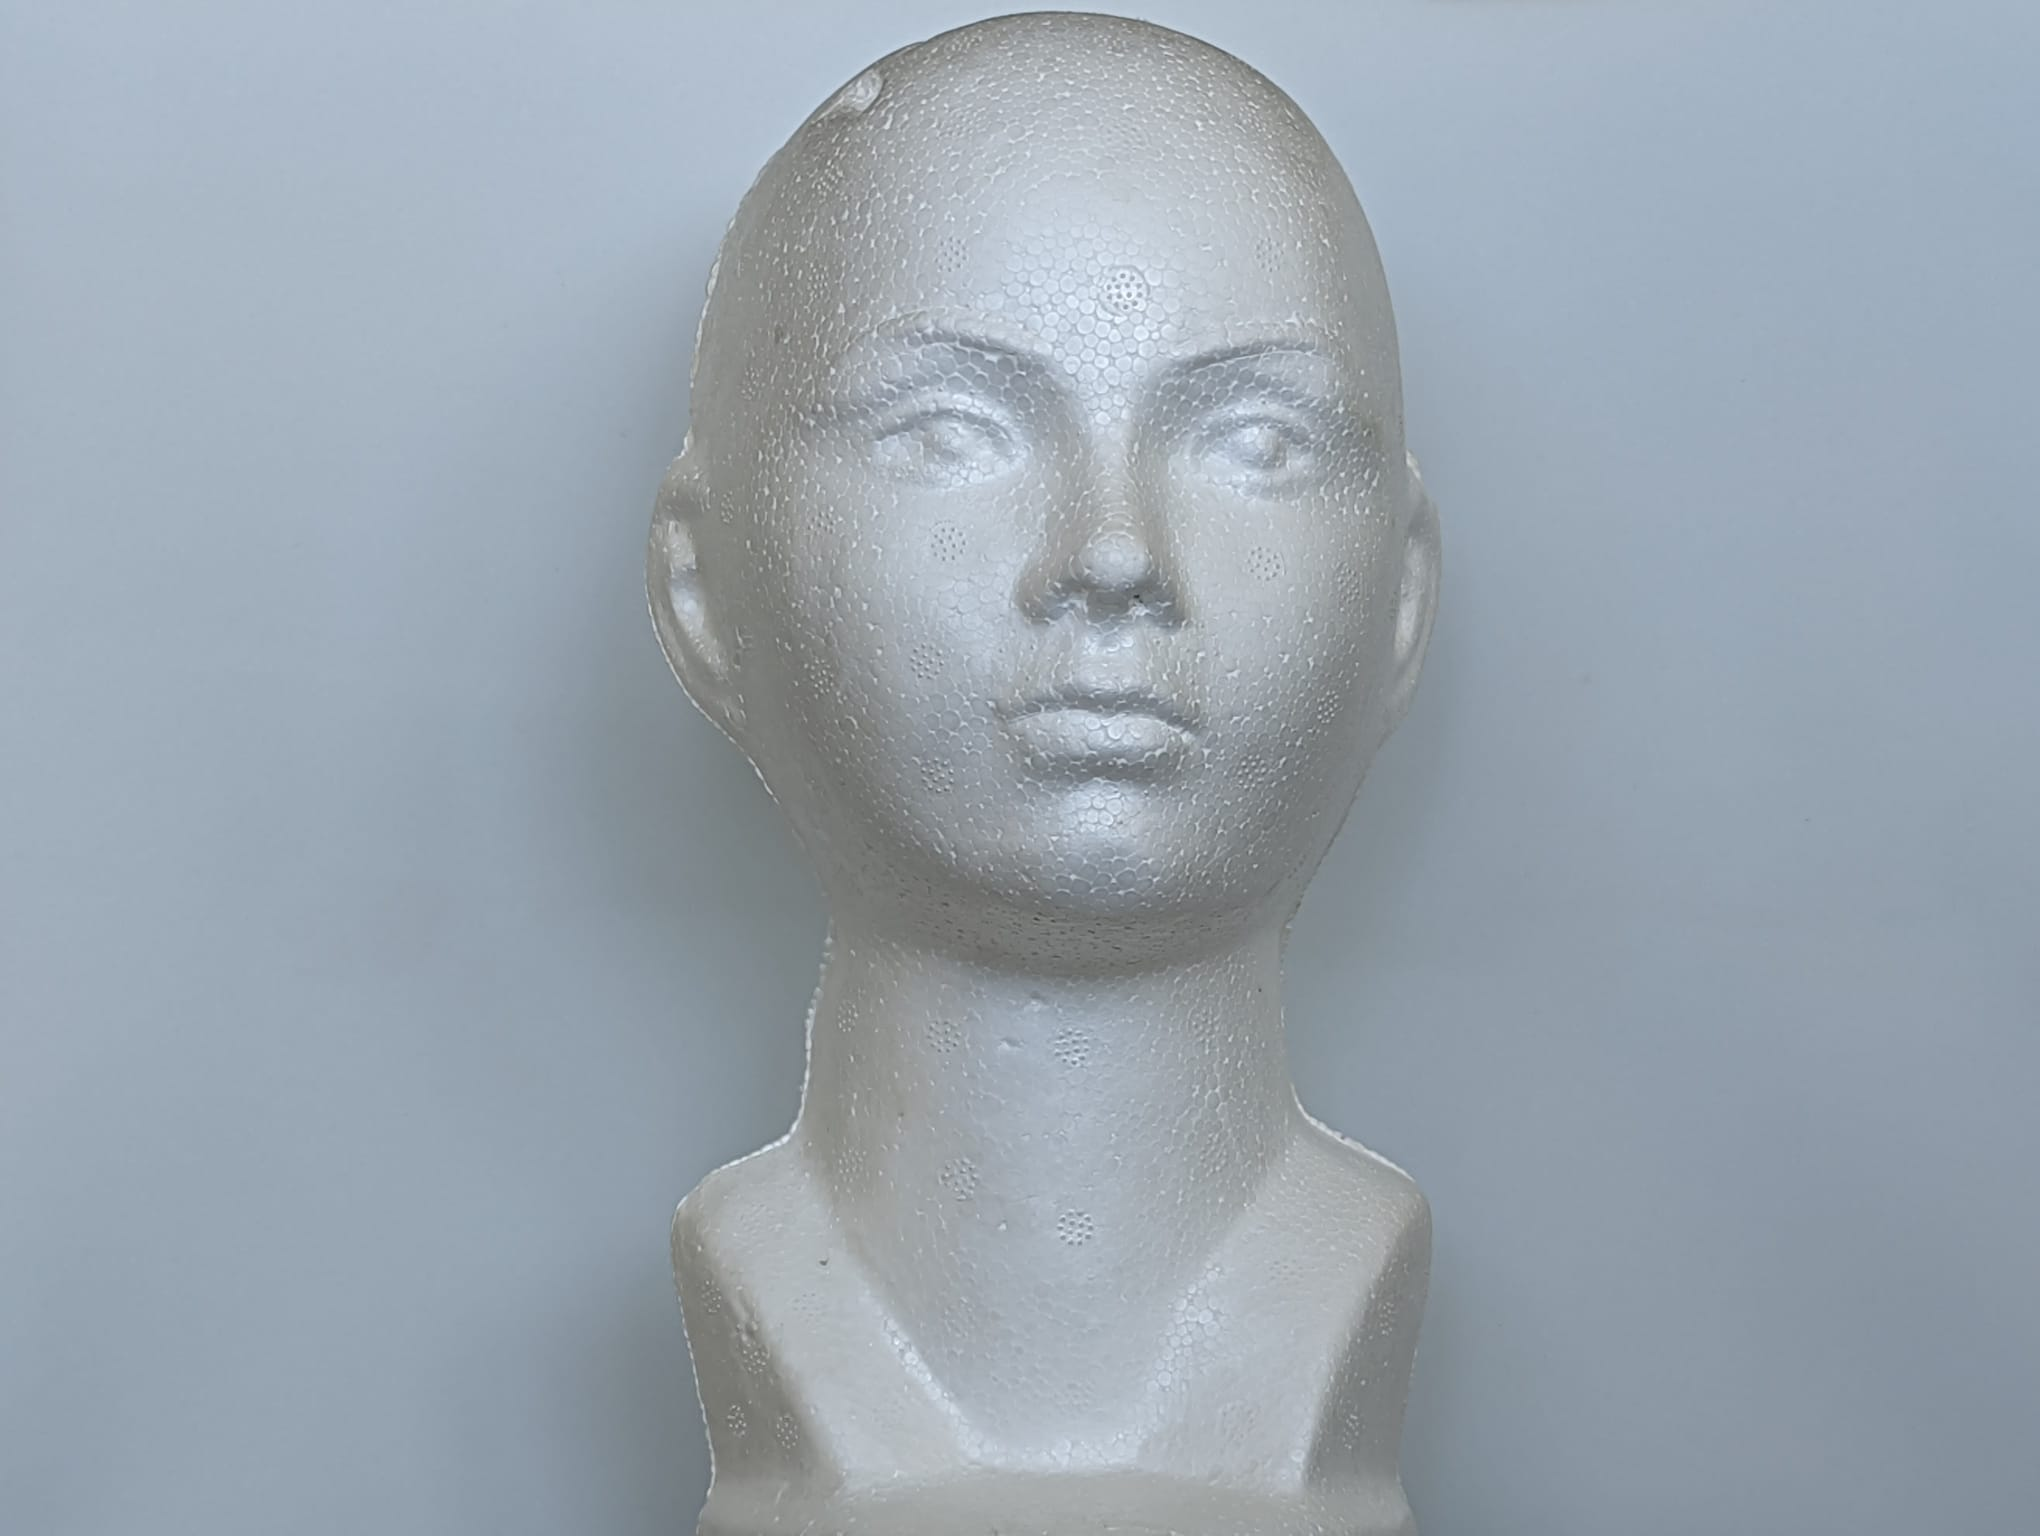
\includegraphics[width=0.3\textwidth]{Figures/Plain_Bust.jpeg}
    \caption{Polystyrene Bust}
    \label{fig:Bust}
\end{figure}

\subsection{SYNTHETIC FRINGES}
It can be shown that optical interference generates sinusoidal fringe patterns. Furthermore, by introducing different polarization's in a beam´s transversal profile it is possible to displace the fringes between zero and $2\pi$. This is done by using a linear polarizer to pick the different polarized states giving the illusion of fringe displacement. Implementing a scanning system like this means that you need an optical arrangement with highly controlled conditions and this is not aligned with the work´s goal. For this reason, the team used synthetic fringes generated by a conventional projector. \\

\begin{figure}[H]
    \centering
    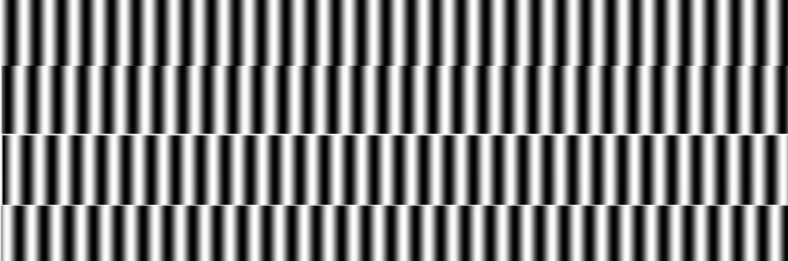
\includegraphics[width=0.4\textwidth]{Figures/Fringe_Disp.jpg}
    \caption{Synthetic Fringes}
    \label{fig:Fringe_Disp}
\end{figure}

Other advantages of using synthetic fringes is the greater control they offer. In particular we are intrested on the orientation, contrast and the spatial frequency ($w = 0.6 cm$). To implement such fringes, the team used the licensed software MATLAB to generate a video that includes the 4 frames of the displaced fringes (Figure \ref{fig:Fringe_Disp}). This video is then uploaded to the projector to further be projected in a scanning session. \\ 

\subsection{EXPERIMENTAL SETUP}
%Fondo blanco mate plano
%Remover ruido exterior
%Fijar puntos para instalacion de busto
%Considerar altura de enfoque
%Parametros experimentales \beta y w

For the experiment, the projector and the nose of the mannequin were adjusted to the same heights at a distance of roughly 1.53 meters of separation between both elements, this distance ensured that the focal point of the projection was at the same level as the ears to guarantee a similar quality of image between the front of the face and the background. The camera was placed below the projector's lens at 1.5 meters from the bust. The angular difference between both ends of the mannequin's face, denoted with the letter $\beta$, varied between 1 and 1.5 degrees. \\

To take the pictures of the bust the stability of the setup was prioritized by reducing the contact with any element of the experiment. Due to the nature of the experiment, the contact with the camera and the bust was inevitable at the moment. To rotate the bust, the team marked the limits in which the bust should stay when rotated. \\

\begin{figure}[H]
    \centering
    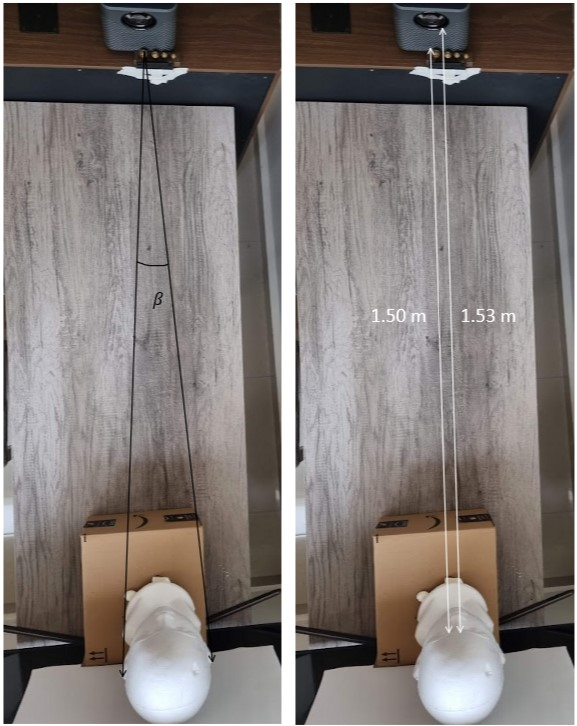
\includegraphics[width=0.3\textwidth, angle =90]{Figures/Exp_Setup.jpg}
    \caption{Experimental Setup}
    \label{fig:Exp_Setup}
\end{figure}

The experimental layout was also designed with the purpose of reducing light noise from the ambient while keeping a clear image free from inside noise caused by the reflection and deformations of the background. This was achieved by covering the top and sides of the setup and by stretching the white background to remove most irregularities on the surface. The background and bust selected for this purpose were both matte white in hopes to reduce the reflective interference to its minimum. \\


\subsection{SURFACE RECONSTRUCTION}
The first step in our method is to obtain the phase of the system. The team used equation \ref{eq:phase} to implement a script that is given the pictures $I_n$ and returns a matrix with the phase values at each point. This phase matrix is visualized in figure \ref{fig:Wrapped_Phase} (b).  

\begin{figure} [H]
     \centering
     \begin{subfigure}[b]{0.22\textwidth}
         \centering
         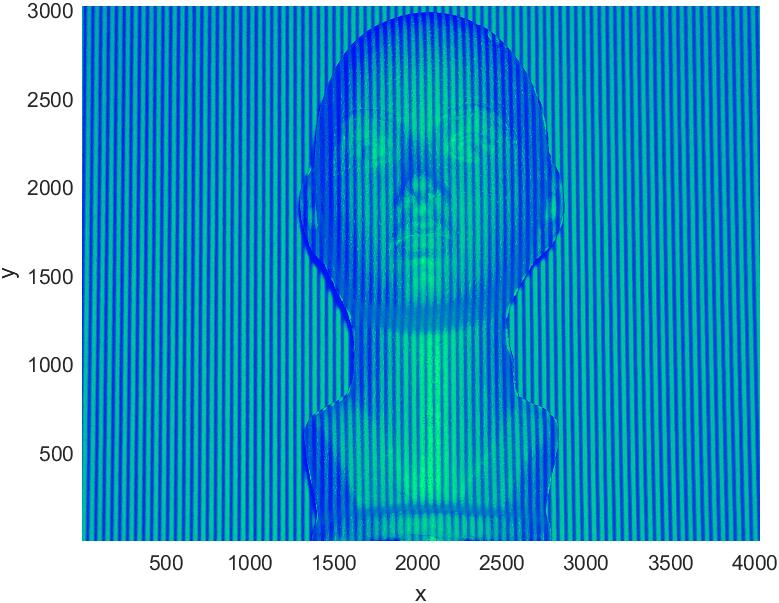
\includegraphics[width=\textwidth]{Figures/Fringe_Imaging.jpg}
         \caption{Fringe Imaging $I_n$}
         \label{fig:Fringe_Imaging}
     \end{subfigure}
     \hfill
     \begin{subfigure}[b]{0.22\textwidth}
         \centering
         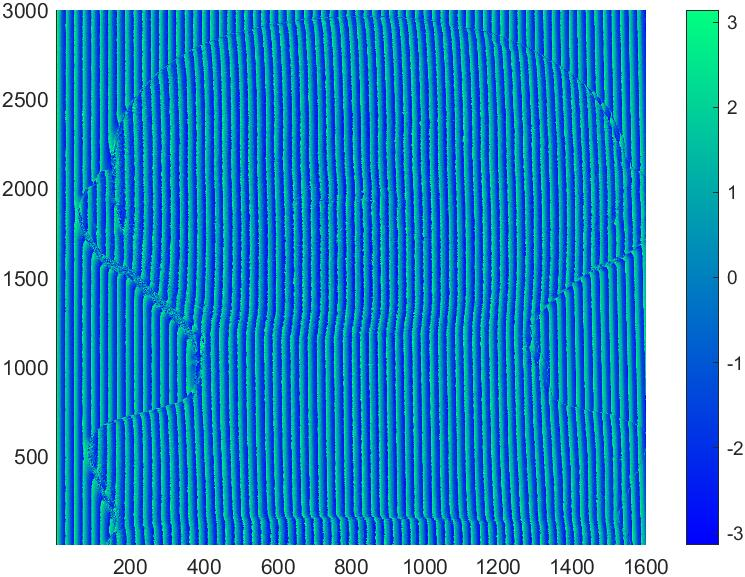
\includegraphics[width=\textwidth]{Figures/Wrapped_Phase.jpg}
         \caption{Phase (Wrapped)}
     \end{subfigure}
        \caption{Phase Measurement}
        \label{fig:Wrapped_Phase}
\end{figure}

After we obtained the wrapped phase of the system, the team used a series of processing algorithms to extract the three dimensional measurements of the object. As discussed in section \ref{sec:TEO_FRAMEWORK}, the phase unwrapping algorithm is critical. %COMO SE LLAMA Y CITA????%%%%%%%%%. 
Unwrapping the phase lead to a result that resembles the object but is tilted as shown in figure \ref{fig:Unwrap_Phase}.

\begin{figure}[H]
    \centering
    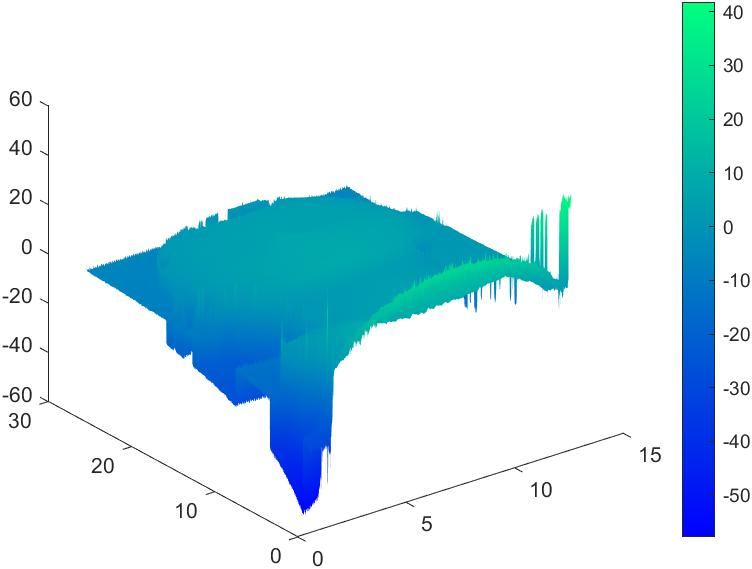
\includegraphics[width=0.2\textwidth]{Figures/Unwrap_Phase.jpg}
    \caption{Unwrapped Phase}
    \label{fig:Unwrap_Phase}
\end{figure}

 The team later related the unwrapped result to the z measurement with equation \ref{eq:topography}. To this result we call the topography of the bust and its also stored in a matrix format. After implementing a numeric filter to smooth the data, the results are the following (Figure \ref{fig:TopBust}):

\begin{figure}[H]
    \centering
    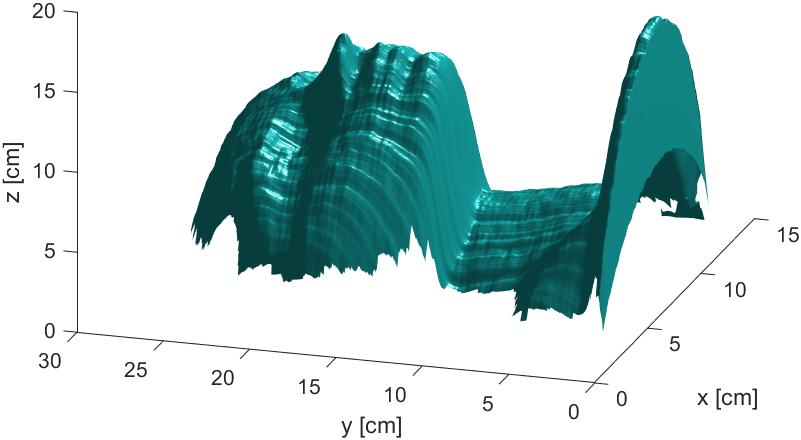
\includegraphics[width=0.4\textwidth]{Figures/Bust_Face.jpg}
    \caption{Topography of the bust}
    \label{fig:TopBust}
\end{figure}

Table 1 shows the quantitative measurements of the bust. From this data the team reports that the measurements deviate from the real value by 0.19 [cm]. This corresponds to a 1.1 $\%$ of relative error. 

\begin{table}[H]
\resizebox{\columnwidth}{!}{ % Scale to column width
\begin{tabular}{|l|l|l|}
\hline
                             & \textbf{Ear to Ear}    & \textbf{Back to Nose}     \\ \hline
Real Value                   & 14.2 {[}cm{]} & 16.4 {[}cm{]}    \\ \hline
Moire by Fringe Displacement & 13 {[}cm{]}   & 16.5937 {[}cm{]} \\ \hline
\end{tabular}
}
\label{tab:Measure}
\caption{Measurements of the Bust}
\end{table}

%Alternative method for 360° scanning
%We tried to implement an alternative for the two mirror 360° \(buscar la referencia del dr rayas) scanning method by rotating the object and dividing it in four sections.
%Esto sería conclusión?

%Four side scanning
%Matrix Superposition Method: hacer un surf con un hold on. (Unir los 4 scans)
%Suavizado

After obtaining the unwrapped, filtered and adjusted reconstruction of each side of the bust the team used a matrix superposition method in which it used the different parts of the simulated mannequin to reconstruct the whole bust. This matrix superposition consists on adjusting the matrix data of each side to be compatible in a single simulation so that each scanned side can fit its designated position. Two variations of this method were applied differing only in the computational simplicity and the exactitude of the final product. \\

\subsubsection{DOUBLE MATRIX RECONSTRUCTION}
%Cabeza back-front 
%Cabeza side1-side2
%Discución de la comparación de ambos resultados
The first variation of the matrix superposition method is called the double matrix reconstruction or two-face reconstruction. This method consists in using the front face and the back of the head of the simulated bust. Both halves would then be adjusted in their spatial position to fit with each other. \\

%%IMAGE OF DOUBLE SIDE RECONS
\begin{figure}[H]
    \centering
    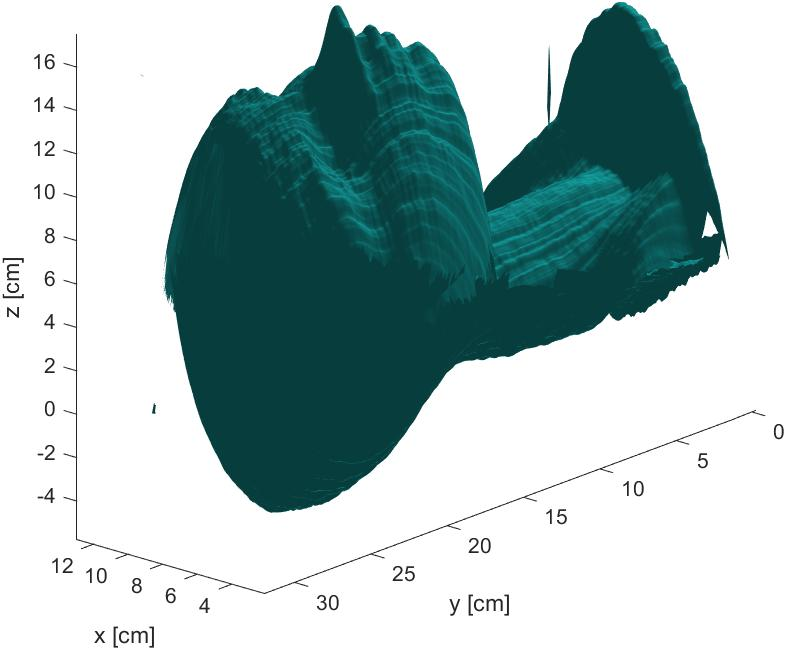
\includegraphics[width=0.35\textwidth]{Figures/Bust_Face_Sidejpg.jpg}
    \caption{Reconstruction using the front and back face of the bust}
    \label{fig:Double}
\end{figure}

The advantage of using only the front and back side of the bust is the simplicity of the reconstruction. In this case the detail on the sides of the bust where not completely lost in the double matrix reconstruction, as seen in figure \ref{fig:Double}, which is fortunate for this simulation. Almost no adjustments were needed to fit both sides together as they were already aligned in the experiment. There was a slight variation in height between the faces due to a deformity in the base of the bust which caused its forward inclination to change when it was rotated. The only disadvantage of this method is that it may loose accuracy in the sides of the reconstructed object. If the object that is scanned is symmetrical or has little to no imperative details on the sides then this method is ideal. \\

\subsubsection{QUADRUPLE MATRIX RECONSTRUCTION}
Countering the double matrix reconstruction discussed earlier, the team came up with the quadruple matrix reconstruction or four-face reconstruction. This method, similar to its counterpart, adjusts the scanned reconstructions of the object in space to make them compatible in a simulation. The quadruple matrix reconstruction uses four scanned sides of the object to offer a more accurate reconstruction of the object. Apart from using the front side and the back side of the object like its homologue, this method implements the lateral sides of the object to bring a more detail to the sides than the double matrix reconstruction method. In figure \ref{fig:Quadruple}, we can see the added detail of the ears in the simulation. \\

%%IMAGE FOUR SIDE RECONS
\begin{figure}[H]
    \centering
    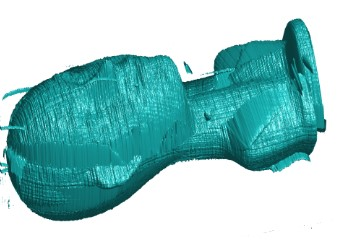
\includegraphics[width=0.35\textwidth]{Figures/FourSideRecons.jpg}
    \caption{Reconstruction using the front, back, left and right sides of the bust}
    \label{fig:Quadruple}
\end{figure}

It is true that this method offers a more precise reconstruction of the original object as it take into account more sections of the same. The principal disadvantages the team found with this method is that the spatial adjustment of the position of the four sides is very complicated using the current tools. The human error made when rotating the object is clearly visible while using this method as the slightest error in the scan can lead to a visible deformity in the simulation. As mentioned before, while processing any side of the object there is noise coming from the background which leads to imperfections in the simulation, this noise and imperfections also collaborate into creating a messy image when combined with the rest of the processed images. If the scanning process gets improved in the future, the four-face reconstruction could prove to be superior than its homologue and there could be even a six-face method where the top and bottom of the object are also implemented into the simulation. \\